%%% PostgreSQL: an Object Relational Database System.
%%%
%%% PostgreSQL is a powerful, open source object-relational database system
%%% with over 30 years of active development that has earned it a strong
%%% reputation for reliability, feature robustness, and performance.
%%%
%%% In this talk we're going to dive into the “object-relational database”
%%% part of this sentence. PostgreSQL was unique in this capabilities when
%%% it was designed, and still is to this day. Spoiler: it has nothing to do
%%% with table inheritance!

\documentclass[xcolor=dvipsnames]{beamer}

\usepackage{minted}

\usepackage{beamerthemesplit}
\usepackage[utf8]{inputenc}
\usepackage[T1]{fontenc}
\usepackage[english]{babel}
\usepackage{calligra}
%% \usepackage{cfr-lm}
\usepackage{tikz}

%% \usepackage{xcolor}

\usepackage{pifont}
\usepackage{newunicodechar}
\newunicodechar{✓}{\ding{51}}
\newunicodechar{✗}{\ding{55}}

\usepackage{csquotes}
\usepackage{ragged2e}

\usetheme{Boadilla}
\setbeamertemplate{itemize items}[square]
\setbeamertemplate{enumerate items}[square]
%\setbeamertemplate{itemize items}{\checkmark}
\beamertemplatenavigationsymbolsempty

\usebackgroundtemplate%
{%
    \begin{tikzpicture}[remember picture,overlay]
      \node[opacity=0.5] at (current page.center) {
        \includegraphics[width=\paperwidth,height=\paperheight]{mammoth-bg.png}%
      };
    \end{tikzpicture}
}

\title{PostgreSQL: an Object Relational Database System.}
\subtitle{PostgreSQL Meetup Paris, 2018}
\author{Dimitri Fontaine}
\institute{CitusData}
\date{June 28, 2018}
%\logo{\includegraphics[height=0.4cm]{logo.png}}

\addtobeamertemplate{frametitle}{}{%
\begin{tikzpicture}[remember picture,overlay]
  \node[anchor=north east,yshift=-6pt] at (current page.north east) {
    \includegraphics[height=0.4cm]{logo-r.png}
  };
\end{tikzpicture}}

%\setbeamercolor{frametitle}{bg=beamer@blendedblue!30}

\begin{document}

\section{Introduction}

\frame{\titlepage}

\begin{frame}[fragile]
  \frametitle{PostgreSQL: an Object Relational Database System.}

  \begin{center}
    %% {\Huge Dimitri Fontaine}
    {\textcalligra{\Huge Dimitri Fontaine}}
    \vfill
    {\Large \textbf{PostgreSQL Major Contributor}}
  \end{center}

\begin{columns}[c]
\column{.5\textwidth} 

  \begin{itemize}
   \item \textbf{pgloader}
   \item \texttt{\textbf{CREATE EXTENSION}}
   \item \texttt{\textbf{CREATE EVENT TRIGGER}}
   \item \textit{Bi-Directional Réplication}
   \item \textit{apt.postgresql.org}
  \end{itemize}  

\column{.5\textwidth}
\begin{center}
  
\includegraphics[height=6em]{postgres-logo.png}
\end{center}
\end{columns}
\end{frame}

\begin{frame}
  \frametitle{Mastering PostgreSQL in Application Development}

  \begin{columns}[c]
    \column{.5\textwidth}
    \begin{minipage}[t][12em][t]{\textwidth}
      \begin{center}
        {\textcalligra{\Huge I wrote a book!}}
      \end{center}
      
      \vfill
      
      \textit{Mastering PostgreSQL in Application Development} teaches SQL
      to developpers: learn to replace thousands of lines of code with
      simple queries.

      \vfill
      \url{http://MasteringPostgreSQL.com}
    \end{minipage}

    \column{.5\textwidth} 
    \begin{center}
      \href{http://MasteringPostgreSQL.com}
           {\includegraphics[height=18em]{MasteringPostgreSQLinAppDev-Cover.png}}
    \end{center}
  \end{columns}
\end{frame}

\section{Glossary}

{
  \usebackgroundtemplate{
    \begin{tikzpicture}[remember picture,overlay]
      \node[opacity=0.35] at (current page.center) {
        \includegraphics[width=\paperwidth,height=\paperheight]{Glossary.jpg}
      };
    \end{tikzpicture}
  }
 
  \begin{frame}
    \frametitle{Glossary}

    \begin{itemize}
    \item Database System
    \item Relational
    \item Object-Relational
    \end{itemize}

  \end{frame}
}


{
  \usebackgroundtemplate{
    \begin{tikzpicture}[remember picture,overlay]
      \node[opacity=0.35] at (current page.center) {
        \includegraphics[width=\paperwidth,height=\paperheight]{network.png}
      };
    \end{tikzpicture}
  }
 
  \begin{frame}
    \frametitle{Database Server}

    \begin{columns}[c]
      \column{.5\textwidth} 

      \begin{itemize}
      \item Concurrency, not storage
      \item ACID
      \item Durability is a thing
      \item Transactions are all about concurrency
      \end{itemize}
      
    \end{columns}

  \end{frame}
}

\begin{frame}
  \frametitle{Storage example: S3 architecture}

  When every concurrent event is its own single file, you don't have
  concurrency issues. Storage is all you need then!

  \begin{center}
    \includegraphics[height=12em]{dp-how-dp-works-v2.png}
  \end{center}

\end{frame}


{
  \usebackgroundtemplate{
    \begin{tikzpicture}[remember picture,overlay]
      \node[opacity=0.15] at (current page.center) {
        \includegraphics[width=\paperwidth,height=\paperheight]
                        {database-schema-1895779_1280-1080x675.png}
      };
    \end{tikzpicture}
  }
 
  \begin{frame}
    \frametitle{Relational}

    \url{https://en.wikipedia.org/wiki/Relation_(database)}

    \vfill

    {
      \LARGE

      In relational database theory, a relation, as originally defined by E.
      F. Codd, is a set of tuples \texttt{(d1, d2, ..., dn)}, where each
      element \texttt{$d_j$} is a member of \texttt{$D_j$}, a data domain. }

  \end{frame}
}

\begin{frame}
  \frametitle{Relational}

  A {\Large relation} is a set of {\Large tuples} where each element is a
  member of a {\Large data domain}, or {\Large data type}:
  
  \begin{center}
    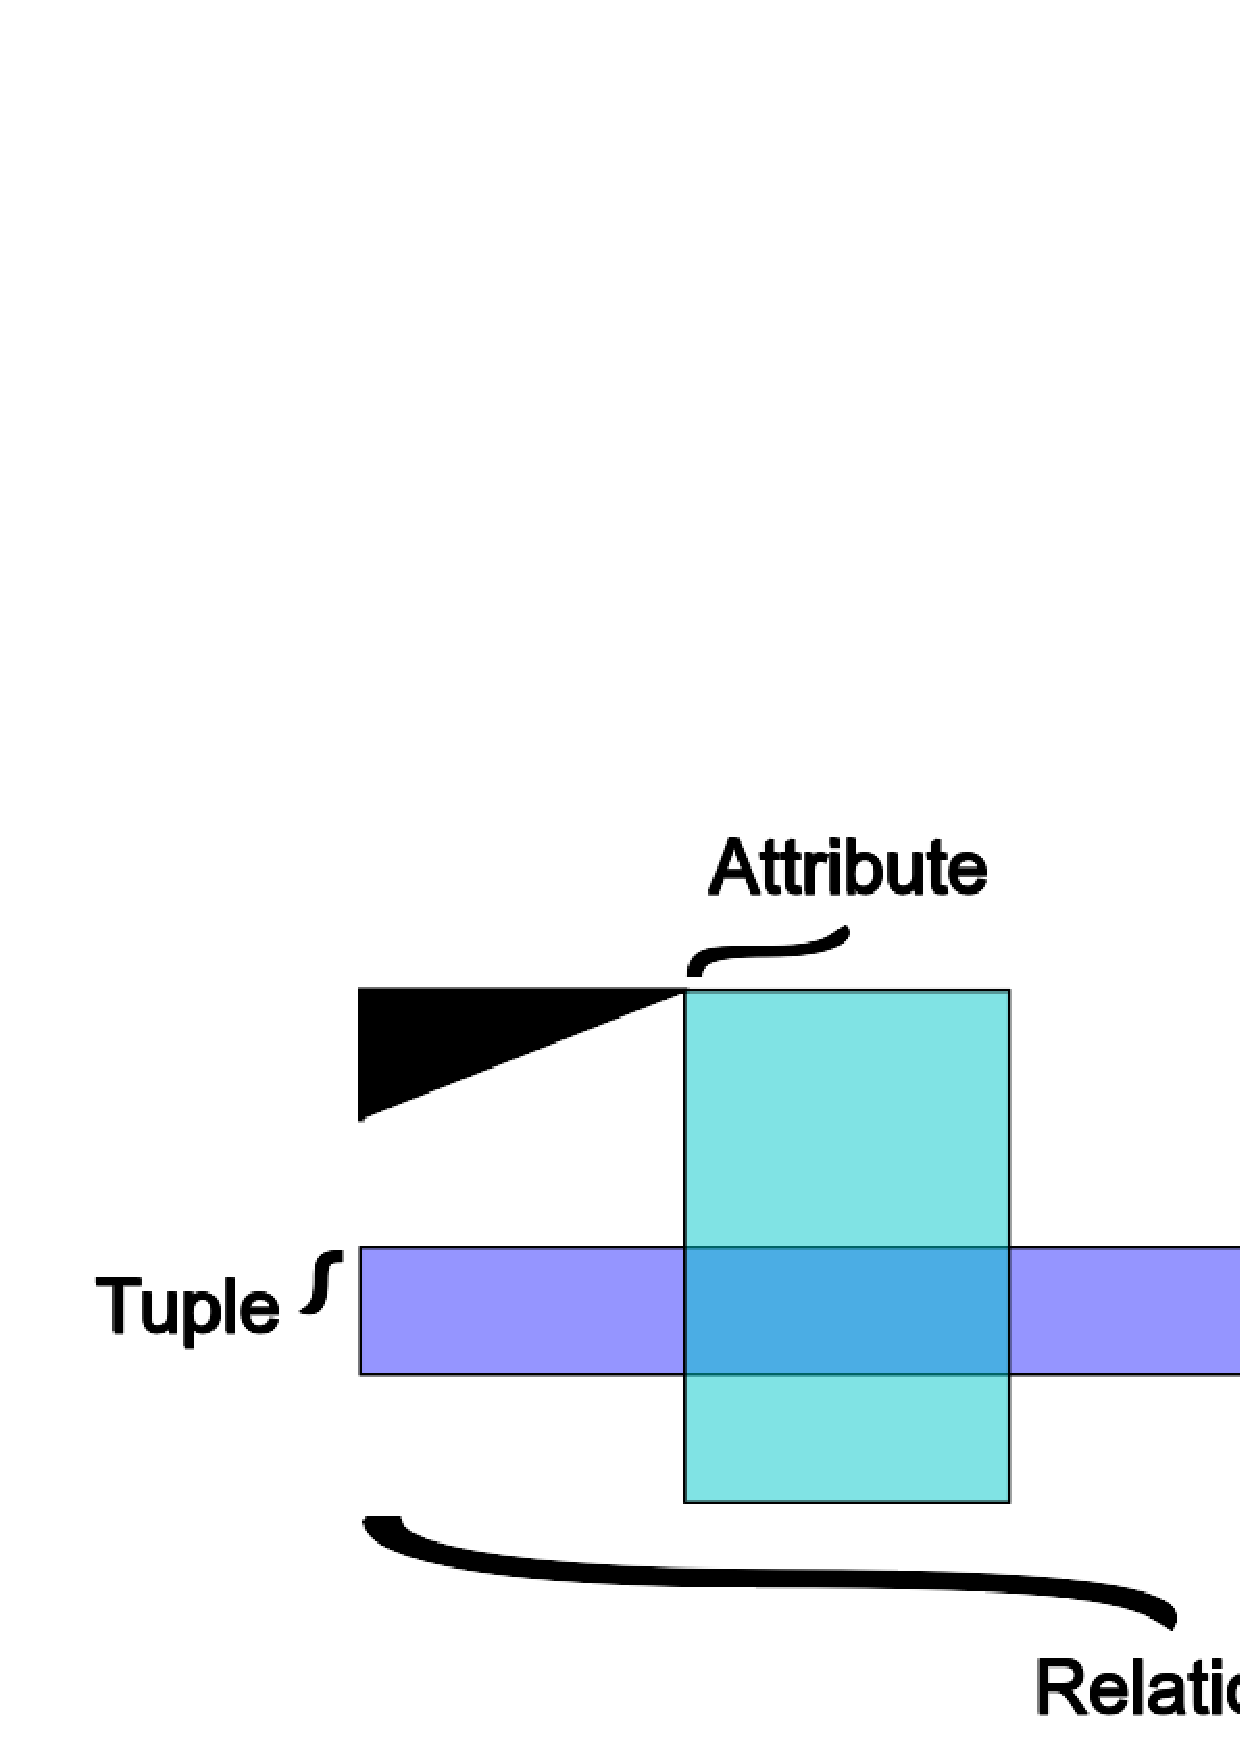
\includegraphics[height=15em] {Relational_database_terms.png}
  \end{center}
  
\end{frame}


{
  \usebackgroundtemplate{
    \begin{tikzpicture}[remember picture,overlay]
      \node at (current page.center) {
        \includegraphics[width=\paperwidth,height=\paperheight]{rj8raf1riyny.png}
      };
    \end{tikzpicture}
  }
 
  \begin{frame}
  \end{frame}
}

{
  %% \usebackgroundtemplate{
  %%   \begin{tikzpicture}[remember picture,overlay]
  %%     \node[opacity=0.25] at (current page.center) {
  %%       %%\includegraphics{square_round.jpg}
  %%       \includegraphics[scale=0.5]{square_round.jpg}
  %%     };
  %%   \end{tikzpicture}
  %% }
 
  \begin{frame}
    \frametitle{Object-Relational}

    \textbf{THE DESIGN OF POSTGRES}, Michael Stonebraker and Lawrence A.
    Rowe. \url{http://db.cs.berkeley.edu/papers/ERL-M85-95.pdf}

    \begin{quote}
    {\scriptsize This paper presents the preliminary design of a new database
      management system, called POSTGRES, that is the successor to the
      INGRES relational database system. The main design goals of the new
      system are to:}
    \end{quote}

    \begin{enumerate}
    \item provide better \textbf{support for complex objects},
    \item provide \textbf{user extendibility for data types, operators and
      access methods},
    \item {\tiny provide facilities for active databases (i.e., alerters and
      triggers) and inferencing includ- ing forward- and backward-chaining,}
    \item {\tiny simplify the DBMS code for crash recovery,}
    \item {\tiny produce a design that can take advantage of optical disks,
      workstations composed of multiple tightly-coupled processors, and
      custom designed VLSI chips, and}
    \item make as few changes as possible (preferably none) to the
      relational model.
    \end{enumerate}

  \end{frame}
}


\section{PostgreSQL Data Types}

\begin{frame}[fragile]
  \frametitle{PostgreSQL Data Types}

  \begin{center}
    \includegraphics[height=15em]{PostgreSQL-Data-Types-300x254.png}
  \end{center}  
\end{frame}

\begin{frame}[fragile]
  \frametitle{Object Reorientation: Generic Functions}

  PostgreSQL data types are known in the catalogs. The following query
  returns a list of them, and that's 73 rows!
  
  \begin{minted}
    [frame=lines,bgcolor=beamer@blendedblue!10,linenos,fontsize=\small]
    {plpgsql}
select nspname, typname
    from      pg_type t
         join pg_namespace n
           on n.oid = t.typnamespace
   where nspname = 'pg_catalog'
     and typname !~ '(^_|^pg_|^reg|_handler$)'
order by nspname, typname;
  \end{minted}
\end{frame}


\begin{frame}[fragile]
  \frametitle{Object Reorientation: Generic Functions}

  \begin{center}
    \includegraphics[height=15em]{multiple-dispatch-julia.jpg}
  \end{center}  
  
\end{frame}


\begin{frame}[fragile]
  \frametitle{Object Reorientation: Generic Functions}

  PostgreSQL provides a complete implementation of function overloading and
  operator overloading and uses it a basis for advanced indexing support:
  
  \begin{minted}
    [frame=lines,bgcolor=beamer@blendedblue!10,linenos,fontsize=\small]
    {plpgsql}
select x, 
       1 + x as "1+",

       '127.0.2.252'::inet + x as "ip address",
       
       set_masklen(('127.0.2.252'::inet + x)::cidr, 28) as "CIDR/28",
       
       date '2016-02-26' + x as date,
       
       cast(date_trunc('month', date '2016-02-26' +x)
         + interval '1 month - 1 day' as date) as "last day"

  from generate_series(0, 6) as t(x);
  \end{minted}
\end{frame}


\begin{frame}[fragile]
  \frametitle{Object Reorientation: Generic Functions}

  PostgreSQL provides a complete implementation of function overloading and
  operator overloading and uses it a basis for advanced indexing support:

  \vfill
  
  \begin{minted}
    [frame=lines,bgcolor=beamer@blendedblue!10,linenos,fontsize=\small]
    {plpgsql}
 x | 1+ | ip address  |    CIDR/28     |    date    |  last day  
---+----+-------------+----------------+------------+------------
 0 |  1 | 127.0.2.252 | 127.0.2.240/28 | 2016-02-26 | 2016-02-29
 1 |  2 | 127.0.2.253 | 127.0.2.240/28 | 2016-02-27 | 2016-02-29
 2 |  3 | 127.0.2.254 | 127.0.2.240/28 | 2016-02-28 | 2016-02-29
 3 |  4 | 127.0.2.255 | 127.0.2.240/28 | 2016-02-29 | 2016-02-29
 4 |  5 | 127.0.3.0   | 127.0.3.0/28   | 2016-03-01 | 2016-03-31
 5 |  6 | 127.0.3.1   | 127.0.3.0/28   | 2016-03-02 | 2016-03-31
 6 |  7 | 127.0.3.2   | 127.0.3.0/28   | 2016-03-03 | 2016-03-31
(7 rows)
  \end{minted}
\end{frame}


\begin{frame}[fragile]
  \frametitle{PostgreSQL Data Types: boolean}

  \begin{columns}[c]
    \column{.5\textwidth}
    \begin{itemize}
    \item Three-Valued Logic
    \item True, False, NULL
    \item NOT NULL Constraints
    \item Boolean Aggregates
    \end{itemize}
    \column{.5\textwidth} 
    \begin{center}
      \includegraphics[height=12em]{boolean-logo.png}
    \end{center}
  \end{columns}
\end{frame}


\begin{frame}[fragile]
  \frametitle{PostgreSQL Data Types: boolean}

  In SQL, boolean implement Three-Valued Logic: \texttt{NULL = NULL} is
  \texttt{NULL}. Here, we see the boolean aggregate \texttt{bool\_and()}:

  \vfill
  
  \begin{minted}
    [frame=lines,bgcolor=beamer@blendedblue!10,linenos,fontsize=\small]
    {plpgsql}
  select year,
         format('%s %s', forename, surname) as name,
         count(*) as ran,
         count(*) filter(where position = 1) as won,
         count(*) filter(where position is not null) as finished,
         sum(points) as points
    from      races
         join results using(raceid)
         join drivers using(driverid)
group by year, drivers.driverid
  having bool_and(position = 1) is true
order by year, points desc;
  \end{minted}
\end{frame}


\begin{frame}[fragile]
  \frametitle{PostgreSQL Data Types: boolean}

  List of drivers who won every race they finished in a given season:

  \vfill
  
  \begin{minted}
    [frame=lines,bgcolor=beamer@blendedblue!10,linenos,fontsize=\scriptsize]
    {plpgsql}
 year |        name         | ran | won | finished | points 
------+---------------------+-----+-----+----------+--------
 1950 | Juan Fangio         |   7 |   3 |        3 |     27
 1950 | Johnnie Parsons     |   1 |   1 |        1 |      9
 1951 | Lee Wallard         |   1 |   1 |        1 |      9
 1952 | Alberto Ascari      |   7 |   6 |        6 |   53.5
 1952 | Troy Ruttman        |   1 |   1 |        1 |      8
 1953 | Bill Vukovich       |   1 |   1 |        1 |      9
 1954 | Bill Vukovich       |   1 |   1 |        1 |      8
 1955 | Bob Sweikert        |   1 |   1 |        1 |      8
 1956 | Pat Flaherty        |   1 |   1 |        1 |      8
 1956 | Luigi Musso         |   4 |   1 |        1 |      5
 1957 | Sam Hanks           |   1 |   1 |        1 |      8
 1958 | Jimmy Bryan         |   1 |   1 |        1 |      8
 1959 | Rodger Ward         |   2 |   1 |        1 |      8
 1960 | Jim Rathmann        |   1 |   1 |        1 |      8
 1961 | Giancarlo Baghetti  |   3 |   1 |        1 |      9
 1966 | Ludovico Scarfiotti |   2 |   1 |        1 |      9
 1968 | Jim Clark           |   1 |   1 |        1 |      9
(17 rows)
  \end{minted}
\end{frame}

\begin{frame}[fragile]
  \frametitle{PostgreSQL Data Types: Text}

  \begin{columns}[c]
    \column{.6\textwidth}
    \begin{itemize}
    \item Text means you know the encoding!
    \item \texttt{client\_encoding}
    \item Pattern-matching (\texttt{like},
      \texttt{{\raise.17ex\hbox{$\scriptstyle\sim$}}})
    \item Text Processing functions
    \item Full Text Search
    \end{itemize}
    \column{.4\textwidth} 
    \begin{center}
      \includegraphics[height=12em]{text-processing-logo.png}
    \end{center}
  \end{columns}
\end{frame}

\begin{frame}[fragile]
  \frametitle{PostgreSQL Data Types: Text}

  PostgreSQL provides advanced text processing:

  \vfill  
  
  \begin{minted}
    [frame=lines,bgcolor=beamer@blendedblue!10,linenos,fontsize=\small]
    {plpgsql}
with categories(id, categories) as
 (
   select id,
          regexp_split_to_array(
            regexp_split_to_table(themes, ','),
            ' > ')
          as categories
     from opendata.archives_planete
 )
 select id,
        categories[1] as category,
        categories[2] as subcategory
   from categories
  where id = 'IF39599';
  \end{minted}
\end{frame}


\begin{frame}[fragile]
  \frametitle{PostgreSQL Data Types: Text}

  PostgreSQL provides functions to process text, even in complex ways. This
  can be used to implement an {\Large ELT} process: Extract, Load in
  PostgreSQL, Transform using SQL.

  \vfill
  
  \begin{minted}
    [frame=lines,bgcolor=beamer@blendedblue!10,linenos,fontsize=\scriptsize]
    {plpgsql}
   id    |         category          |       subcategory        
---------+---------------------------+--------------------------
 IF39599 | Habillement               | Habillement traditionnel
 IF39599 | Etres humains             | Homme
 IF39599 | Etres humains             | Portrait
 IF39599 | Relations internationales | Présence étrangère
(4 rows)
  \end{minted}
\end{frame}


\begin{frame}[fragile]
  \frametitle{PostgreSQL Data Types: Date and Time}

  \begin{columns}[c]
    \column{.6\textwidth}
    \begin{itemize}
    \item \texttt{Timestamp with Time Zone}
    \item \texttt{Interval}
    \item Year Zero doesn't exist in our calendar!
    \item Remember that \texttt{between} is an inclusive operator
    \item \texttt{date\_trunc}, \texttt{extract}, \texttt{to\_char}, ...
    \end{itemize}
    \column{.4\textwidth} 
    \begin{center}
      \includegraphics[height=12em]{time_sheduled-512.png}
    \end{center}
  \end{columns}
\end{frame}


\begin{frame}[fragile]
  \frametitle{PostgreSQL Data Types: Date and Time}

  Here an example of date based reporting:
  
  \vfill
  
  \begin{minted}
    [frame=lines,bgcolor=beamer@blendedblue!10,linenos,fontsize=\small]
    {plpgsql}
  select extract(isodow from ats) as dow,
         to_char(ats, 'Day') as day,
         count(*) as commits,
         round(100.0*count(*)/sum(count(*)) over(), 2) as pct,
         repeat('*', (100*count(*)/sum(count(*)) over())::int) as hist
    from commitlog
   where project = 'postgres'
group by dow, day
order by dow;
  \end{minted}
\end{frame}


\begin{frame}[fragile]
  \frametitle{PostgreSQL Data Types: Date and Time}

  Producing an histogram in SQL is that easy:
  
  \vfill
  
  \begin{minted}
    [frame=lines,bgcolor=beamer@blendedblue!10,linenos,fontsize=\small]
    {plpgsql}
 dow |    day    | commits |  pct  |       hist       
-----+-----------+---------+-------+------------------
   1 | Monday    |    6746 | 15.06 | ***************
   2 | Tuesday   |    7376 | 16.46 | ****************
   3 | Wednesday |    6759 | 15.09 | ***************
   4 | Thursday  |    7357 | 16.42 | ****************
   5 | Friday    |    7276 | 16.24 | ****************
   6 | Saturday  |    4855 | 10.84 | ***********
   7 | Sunday    |    4434 |  9.90 | **********
(7 rows)
  \end{minted}
\end{frame}

{
  \usebackgroundtemplate{
    \begin{tikzpicture}[remember picture,overlay]
      \node[opacity=1] at (current page.center) {
        \includegraphics[width=\paperwidth,height=\paperheight]{hist.png}
      };
    \end{tikzpicture}
  }
 
  \begin{frame}
    \frametitle {}

  \end{frame}
}


\begin{frame}[fragile]
  \frametitle{PostgreSQL Data Types: Network Addresses}

  \begin{columns}[c]
    \column{.6\textwidth}
    \begin{itemize}
    \item \texttt{cidr}, texttt{inet}, \texttt{macaddr}
    \item Support both ipv4 and ipv6
    \item Classic use case: web server logs
    \item See also \url{https://github.com/RhodiumToad/ip4r}
    \end{itemize}
    \column{.4\textwidth} 
    \begin{center}
      \includegraphics[height=12em]{Network-Ip-Address-icon.png}
    \end{center}
  \end{columns}
\end{frame}


\begin{frame}[fragile]
  \frametitle{PostgreSQL Data Types: Network Addresses}

  Here, we analyze network traffic per origin subnet:
  
  \vfill
  
  \begin{minted}
    [frame=lines,bgcolor=beamer@blendedblue!10,linenos,fontsize=\small]
    {plpgsql}
  select set_masklen(ip::cidr, 24) as network,
         count(*) as requests,
         array_length(array_agg(distinct ip), 1) as ipcount
    from access_log
group by network
  having array_length(array_agg(distinct ip), 1) > 1
order by requests desc, ipcount desc;
  \end{minted}
\end{frame}


\begin{frame}[fragile]
  \frametitle{PostgreSQL Data Types: Network Addresses}

  The previous query aggregates requests per IP subnets:

  \vfill
  
  \begin{minted}
    [frame=lines,bgcolor=beamer@blendedblue!10,linenos,fontsize=\scriptsize]
    {plpgsql}
     network      | requests | ipcount 
------------------+----------+---------
 4.152.207.0/24   |      140 |       2
 222.95.35.0/24   |       59 |       2
 211.59.0.0/24    |       32 |       2
 61.10.7.0/24     |       25 |      25
 222.166.160.0/24 |       25 |      24
 219.153.10.0/24  |        7 |       3
 218.78.209.0/24  |        6 |       4
 193.109.122.0/24 |        5 |       5
 204.102.106.0/24 |        3 |       3
 66.134.74.0/24   |        2 |       2
 219.133.137.0/24 |        2 |       2
 61.180.25.0/24   |        2 |       2
(12 rows)
  \end{minted}
\end{frame}


\begin{frame}[fragile]
  \frametitle{PostgreSQL Data Types: Ranges}

  \begin{columns}[c]
    \column{.6\textwidth}
    \begin{itemize}
    \item Two dimensions in a single column
    \item Support for overlapping! \texttt{\&\&}
    \item \texttt{exclude using gist (currency with =, validity with \&\&)}
    \item Validity periods, history tables
    \item Classic example: VAT
    \end{itemize}
    \column{.4\textwidth} 
    \begin{center}
      \includegraphics[height=12em]{reloading-timer-clock-icon-by-vexels.png}
    \end{center}
  \end{columns}
\end{frame}


\begin{frame}[fragile]
  \frametitle{PostgreSQL Data Types: Ranges}

  Here we use range to have a single valid value for an exchange rate given
  a calendar date:
  
  \vfill
  
  \begin{minted}
    [frame=lines,bgcolor=beamer@blendedblue!10,linenos,fontsize=\small]
    {plpgsql}
select rate
  from rates
 where currency = 'Euro' 
 and validity @> date '2017-05-18';
  \end{minted}
\end{frame}


\begin{frame}[fragile]
  \frametitle{PostgreSQL Data Types: Ranges}

  The Euro rate for 2017-05-18 is unique, thanks to our non-overlapping
  constraint. The expression \texttt{validity @> date} could be used in a
  join.

  \vfill
  
  \begin{minted}
    [frame=lines,bgcolor=beamer@blendedblue!10,linenos,fontsize=\small]
    {plpgsql}
   rate   
----------
 1.240740
(1 row)
  \end{minted}
\end{frame}


\begin{frame}[fragile]
  \frametitle{PostgreSQL Data Types: Arrays}

  \begin{columns}[c]
    \column{.6\textwidth}
    \begin{itemize}
    \item Denormalization technique: lookup table
    \item GIN indexes, when searching contents
    \item \texttt{unnest} and \texttt{lateral}
    \end{itemize}
    \column{.4\textwidth} 
    \begin{center}
      \includegraphics[height=12em]{matrix.png}
    \end{center}
  \end{columns}
\end{frame}


\begin{frame}[fragile]
  \frametitle{PostgreSQL Data Types: Arrays}

  Here, we build arrays from a free-form data set:
  
  \vfill
  
  \begin{minted}
    [frame=lines,bgcolor=beamer@blendedblue!10,linenos,fontsize=\small]
    {plpgsql}
with matches as (
  select id,
         regexp_matches(message, '(#[^ ,]+)', 'g') as match
    from tweet
),
    hashtags as (
  select id,
         array_agg(match[1] order by match[1]) as hashtags
    from matches
group by id
)      
  \end{minted}
\end{frame}


\begin{frame}[fragile]
  \frametitle{PostgreSQL Data Types: Arrays}

  The insert part of the query:

  \vfill
  
  \begin{minted}
    [frame=lines,bgcolor=beamer@blendedblue!10,linenos,fontsize=\small]
    {plpgsql}
insert into hashtag(id, date, uname, message, location, hashtags)
     select id,
            date + hour as date,
            uname,
            message,
            point(longitude, latitude),
            hashtags
       from      hashtags
       join tweet using(id);
  \end{minted}
\end{frame}


\begin{frame}[fragile]
  \frametitle{PostgreSQL Data Types: Arrays}

  When using the whole content of an array, use \texttt{unnest}:

  \vfill
  
  \begin{minted}
    [frame=lines,bgcolor=beamer@blendedblue!10,linenos,fontsize=\small]
    {plpgsql}
  select tag, count(*)
    from hashtag, unnest(hashtags) as t(tag)
group by tag
order by count desc
   limit 10;
  \end{minted}
\end{frame}


\begin{frame}[fragile]
  \frametitle{PostgreSQL Data Types: Arrays}

  The \texttt{unnest} function allows to apply classic SQL to filter the
  array contents, including joins:
  
  \vfill
  
  \begin{minted}
    [frame=lines,bgcolor=beamer@blendedblue!10,linenos,fontsize=\small]
    {plpgsql}
     tag      | count 
--------------+-------
 #Hiring      | 37964
 #Jobs        | 24776
 #CareerArc   | 21845
 #Job         | 21368
 #job         | 17763
 #Retail      |  7867
 #Hospitality |  7664
 #job?        |  7569
 #hiring!     |  6860
 #Job:        |  5953
(10 rows)
\end{minted}
\end{frame}

\begin{frame}[fragile]
  \frametitle{PostgreSQL Data Types: Arrays}

  Search for \texttt{\#Hiring} in \texttt{\#Retail} per geolocation:

  \vfill
  
  \begin{minted}
    [frame=lines,bgcolor=beamer@blendedblue!10,linenos,fontsize=\scriptsize]
    {plpgsql}
  select name,
         substring(timezone, '/(.*)') as tz,
         count(*)
    from hashtag
    
         left join lateral
         (
            select *
              from geonames
          order by location <-> hashtag.location
             limit 1
         )
         as geoname
         on true
  
   where hashtags @> array['#Hiring', '#Retail']
   
group by name, tz
order by count desc
   limit 10;
  \end{minted}
\end{frame}

\begin{frame}[fragile]
  \frametitle{PostgreSQL Data Types: Arrays}

  Search for \texttt{\#Hiring} in \texttt{\#Retail} per geolocation:

  \vfill
  
  \begin{minted}
    [frame=lines,bgcolor=beamer@blendedblue!10,linenos,fontsize=\scriptsize]
    {plpgsql}
                       name                       |     tz      | count 
--------------------------------------------------+-------------+-------
 San Jose City Hall                               | Los_Angeles |    31
 Sleep Inn & Suites Intercontinental Airport East | Chicago     |    19
 Los Angeles                                      | Los_Angeles |    14
 Dallas City Hall Plaza                           | Chicago     |    12
 New York City Hall                               | New_York    |    11
 Jw Marriott Miami Downtown                       | New_York    |    11
 Gold Spike Hotel & Casino                        | Los_Angeles |    10
 San Antonio                                      | Chicago     |    10
 Shoppes at 104                                   | New_York    |     9
 Fruitville Elementary School                     | New_York    |     8
(10 rows)
  \end{minted}
\end{frame}

\begin{frame}[fragile]
  \frametitle{PostgreSQL Data Types: XML}

  \begin{columns}[c]
    \column{.6\textwidth}
    \begin{itemize}
    \item SQL standard
    \item Manage XML documents
    \item Not feature complete
    \item \texttt{PL/XSLT}
    \end{itemize}
    \column{.4\textwidth} 
    \begin{center}
      \includegraphics[height=12em]{XML-icon.png}
    \end{center}
  \end{columns}
\end{frame}


\begin{frame}[fragile]
  \frametitle{PostgreSQL Data Types: XML}

  Processing XML right from inside your database thanks to PL/XSLT:

  \vfill
  
  \begin{minted}
    [frame=lines,bgcolor=beamer@blendedblue!10,linenos,fontsize=\scriptsize]
    {plpgsql}
create extension plxslt;

CREATE OR REPLACE FUNCTION striptags(xml) RETURNS text
	LANGUAGE xslt
AS $$<?xml version="1.0"?>
<xsl:stylesheet version="1.0"
    xmlns:xsl="http://www.w3.org/1999/XSL/Transform"
    xmlns="http://www.w3.org/1999/xhtml"
>

  <xsl:output method="text" omit-xml-declaration="yes"/>

  <xsl:template match="/">
    <xsl:apply-templates/>
  </xsl:template>

</xsl:stylesheet>
$$;    
  \end{minted}
\end{frame}


\begin{frame}[fragile]
  \frametitle{PostgreSQL Data Types: XML}

  \begin{minted}
    [frame=lines,bgcolor=beamer@blendedblue!10,linenos,fontsize=\normalsize]
    {plpgsql}
create table docs
 (
   id      serial primary key,
   content xml
 );

insert into docs(content)
     values ('<?xml version="1.0"?>
<html xmlns="http://www.w3.org/1999/xhtml">
<body>hello</body>
</html>');

select id, striptags(content)
  from docs;
  \end{minted}
\end{frame}


\begin{frame}[fragile]
  \frametitle{PostgreSQL Data Types: XML}

  It just works, of course:

  \vfill
  
  \begin{minted}
    [frame=lines,bgcolor=beamer@blendedblue!10,linenos,fontsize=\normalsize]
    {plpgsql}
 id | striptags 
----+-----------
  1 |          
    | hello    
    | 
(1 row)
  \end{minted}
\end{frame}

\begin{frame}[fragile]
  \frametitle{PostgreSQL Data Types: JSON}

  \begin{columns}[c]
    \column{.6\textwidth}
    \begin{itemize}
    \item The new document format
    \item Advanced support in PostgreSQL
    \item Indexing and search
    \item Producing JSON from queries
    \end{itemize}
    \column{.4\textwidth} 
    \begin{center}
      \includegraphics[height=12em]{json-logo.png}
    \end{center}
  \end{columns}
\end{frame}


\begin{frame}[fragile]
  \frametitle{PostgreSQL Data Types: JSON}

  Using \textit{Magic: the Gathering} data in JSON:

  \vfill
  
  \begin{minted}
    [frame=lines,bgcolor=beamer@blendedblue!10,linenos,fontsize=\normalsize]
    {plpgsql}
  select data->'colors' as colors,
         count(*)
    from magic.cards
   where data @> '{"colors": ["White","Blue","Black"]}'
group by grouping sets(data->'colors', ())
order by count desc;  \end{minted}
\end{frame}


\begin{frame}[fragile]
  \frametitle{PostgreSQL Data Types: JSON}

  Searching JSON data in PostgreSQL is easy:

  \vfill
  
  \begin{minted}
    [frame=lines,bgcolor=beamer@blendedblue!10,linenos,fontsize=\normalsize]
    {plpgsql}
                   colors                   | count 
--------------------------------------------+-------
 ¤                                          |    98
 ["White", "Blue", "Black"]                 |    57
 ["White", "Blue", "Black", "Red", "Green"] |    37
 ["White", "Blue", "Black", "Red"]          |     2
 ["White", "Blue", "Black", "Green"]        |     2
(5 rows)
  \end{minted}
\end{frame}

\begin{frame}[fragile]
  \frametitle{PostgreSQL Data Types: ENUM}

  \begin{columns}[c]
    \column{.6\textwidth}
    \begin{itemize}
    \item Non standard
    \item Makes it easy to switch from MySQL
    \item Avoid lookup tables
    \item Great when you know set of values will \textbf{never} change.
    \end{itemize}
    \column{.4\textwidth} 
    \begin{center}
      \includegraphics[height=12em]{shop_set-31-512.png}
    \end{center}
  \end{columns}
\end{frame}


\begin{frame}[fragile]
  \frametitle{PostgreSQL Data Types: ENUM}

  A data model that could be using ENUM... but is not... yet:

  \vfill
  
  \begin{minted}
    [frame=lines,bgcolor=beamer@blendedblue!10,linenos,fontsize=\normalsize]
    {plpgsql}
create table color(id serial primary key, name text);

create table cars
 (
   brand   text,
   model   text,
   color   integer references color(id)
 );

insert into color(name)
     values ('blue'), ('red'),
     ('gray'), ('black');
  \end{minted}
\end{frame}


\begin{frame}[fragile]
  \frametitle{PostgreSQL Data Types: ENUM}

  Joining at \texttt{INSERT} time:

  \vfill
  
  \begin{minted}
    [frame=lines,bgcolor=beamer@blendedblue!10,linenos,fontsize=\normalsize]
    {plpgsql}
insert into cars(brand, model, color)
     select brand, model, color.id
      from (
            values('ferari', 'testarosa', 'red'),
                  ('aston martin', 'db2', 'blue'),
                  ('bentley', 'mulsanne', 'gray'),
                  ('ford', 'T', 'black')
           )
             as data(brand, model, color)
           join color on color.name = data.color;
  \end{minted}
\end{frame}


\begin{frame}[fragile]
  \frametitle{PostgreSQL Data Types: ENUM}

  The ENUM variant of the data model:

  \vfill
  
  \begin{minted}
    [frame=lines,bgcolor=beamer@blendedblue!10,linenos,fontsize=\footnotesize]
    {plpgsql}
create type color_t as enum('blue', 'red', 'gray', 'black');

drop table if exists cars;
create table cars
 (
   brand   text,
   model   text,
   color   color_t
   );

insert into cars(brand, model, color)
  values ('ferari', 'testarosa', 'red'),
         ('aston martin', 'db2', 'blue'),
         ('bentley', 'mulsanne', 'gray'),
         ('ford', 'T', 'black');
  \end{minted}
\end{frame}

\begin{frame}[fragile]
  \frametitle{PostgreSQL Data Types: Point}

  \begin{columns}[c]
    \column{.6\textwidth}
    \begin{itemize}
    \item Geometry, not geography!
    \item Two-dimensional data type
    \item kNN searches
    \item GiST and SP-GiST indexes
    \item See also PostGIS
    \end{itemize}
    \column{.4\textwidth} 
    \begin{center}
      \includegraphics[height=12em]{earth-tz-logo.jpg}
    \end{center}
  \end{columns}
\end{frame}


\begin{frame}[fragile]
  \frametitle{PostgreSQL Data Types: Point}

  Example of a kNN search to geolocate a sample of tweets:

  \vfill
  
  \begin{minted}
    [frame=lines,bgcolor=beamer@blendedblue!10,linenos,fontsize=\scriptsize]
    {plpgsql}
  select id,
         round((hashtag.location <-> geoname.location)::numeric, 3) as dist,
         country.iso,
         region.name as region,
         district.name as district
    from hashtag
         left join lateral
         (
            select geonameid, isocode, regcode, discode, location
              from geoname.geoname
          order by location <-> hashtag.location
             limit 1
         )
         as geoname
         on true
         left join geoname.country using(isocode)
         left join geoname.region using(isocode, regcode)
         left join geoname.district using(isocode, regcode, discode)
order by id
   limit 10;
  \end{minted}
\end{frame}


\begin{frame}[fragile]
  \frametitle{PostgreSQL Data Types: Point}

  Example of a kNN search to geolocate a sample of tweets:

  \vfill
  
  \begin{minted}
    [frame=lines,bgcolor=beamer@blendedblue!10,linenos,fontsize=\scriptsize]
    {plpgsql}
         id         | dist  | iso |     region     |        district        
--------------------+-------+-----+----------------+------------------------
 720553447402160128 | 0.016 | US  | Florida        | Orange County
 720553457015324672 | 0.018 | US  | Texas          | Smith County
 720553458596757504 | 0.011 | US  | Florida        | Orange County
 720553466804989952 | 0.009 | US  | Pennsylvania   | Philadelphia County
 720553475923271680 | 0.005 | US  | New York       | Nassau County
 720553508190052352 | 0.015 | US  | New York       | Suffolk County
 720553522966581248 | 0.034 | US  | Maryland       | Prince George County
 720553530088669185 | 0.021 | US  | New York       | Rockland County
 720553531665682434 | 0.054 | US  | South Carolina | York County
 720553532273795072 | 0.052 | US  | Nebraska       | Douglas County
(10 rows)
  \end{minted}
\end{frame}

\begin{frame}[fragile]
  \frametitle{PostgreSQL Data Types}

  \begin{center}
    \includegraphics[height=15em]{PostgreSQL-Data-Types-300x254.png}
  \end{center}  
\end{frame}

\begin{frame}[fragile]
  \frametitle{PostgreSQL Data Types: Recap}

  We saw some of the PostgreSQL data types, skipping numeric based types and
  sequences, and some others too. Remember, you can find 73 data types in
  the distribution!

  \vfill

  \begin{columns}[c]
    \column{.5\textwidth}
    \begin{itemize}
    \item Boolean
    \item Text
    \item Date and Time
    \item Network Addresses
    \item Point
    \end{itemize}

    \column{.3\textwidth}
    \begin{itemize}
    \item Ranges
    \item Arrays
    \item XML
    \item JSON
    \item ENUM
    \end{itemize}
  \end{columns}
\end{frame}


\section{Extensions}

{
  \usebackgroundtemplate{
    \begin{tikzpicture}[remember picture,overlay]
      \node[opacity=1] at (current page.center) {
        \includegraphics[width=\paperwidth,\paperheight] {nosql-bigdata.png}
      };
    \end{tikzpicture}
  }
 
  \begin{frame}
    \frametitle{PostgreSQL is YeSQL!}

  \end{frame}
}

{
  \usebackgroundtemplate{
    \begin{tikzpicture}[remember picture,overlay]
      \node[opacity=0.15] at (current page.center) {
        \includegraphics[width=0.8\paperwidth,height=0.8\paperheight]{extensible.jpg}
      };
    \end{tikzpicture}
  }
 
  \begin{frame}
    \frametitle{PostgreSQL Extensions}

    PostgreSQL provide user extendibility for data types, operators and
    access methods.

    \vfill

    \begin{columns}[c]
      \column{.8\textwidth}
      \begin{itemize}
      \item Data Types can be added to PostgreSQL at run time
      \item Write an extension in C
      \item Operators are found dynamically in the catalogs
      \item Index support too: btree, GIN, GiST, SP-Gist, Hash
      \item Extended index support: bloom, RUM
      \end{itemize}
    \end{columns}    
  \end{frame}
}

{
  \usebackgroundtemplate{
    \begin{tikzpicture}[remember picture,overlay]
      \node[opacity=0.15] at (current page.center) {
        \includegraphics[width=0.8\paperwidth,height=0.8\paperheight]{extensible.jpg}
      };
    \end{tikzpicture}
  }
 
  \begin{frame}
    \frametitle{PostgreSQL Extensions}

    Some useful data type extensions for PostgreSQL, found in contrib:

    \vfill

    \begin{columns}[c]
      \column{\textwidth}
      \begin{itemize}
      \item \texttt{bloom}: index access method based on Bloom filters
      \item \texttt{btree\_gin}: sample GIN operator classes that implement B-tree equivalent
      \item \texttt{btree\_gist}: sample GiST operator classes that implement B-tree equivalent
      \item \texttt{earthdistance}: calculating great circle distances on
        the surface of the Earth
      \item \texttt{hstore}: storing sets of key/value pairs
      \item \texttt{intarray}: searching and indexing arrays of integers
      \item \texttt{ltree}: representing labels of data stored in a hierarchical tree-like structure
      \item \texttt{pg\_trgm}: determining the similarity of alphanumeric text based on trigram matching
      \end{itemize}
    \end{columns}    
  \end{frame}
}

{
  \usebackgroundtemplate{
    \begin{tikzpicture}[remember picture,overlay]
      \node[opacity=0.15] at (current page.center) {
        \includegraphics[width=0.8\paperwidth,height=0.8\paperheight]{extensible.jpg}
      };
    \end{tikzpicture}
  }
 
  \begin{frame}
    \frametitle{PostgreSQL Extensions}

    Some useful data type extensions for PostgreSQL, elsewhere:

    \vfill

    \begin{columns}[c]
      \column{.8\textwidth}
      \begin{itemize}
      \item PostGIS: a full GIS system
      \item ip4r: efficient lookup in ranges of ip addresses
      \item hll: HyperLogLog for fuzzy distinct counts
      \item prefix: inverted range lookups
      \item debversion: comparison rules for Debian version strings
      \end{itemize}
    \end{columns}    
  \end{frame}
}


\section{Concusion}

{
  \usebackgroundtemplate{
    \begin{tikzpicture}[remember picture,overlay]
      \node[opacity=1] at (current page.center) {
        
\includegraphics[width=0.5\paperwidth,0.5\paperheight]{postgres-logo.eps}
      };
    \end{tikzpicture}
  }
 
  \begin{frame}
    \frametitle{PostgreSQL is YeSQL!}

  \end{frame}
}


{
  \usebackgroundtemplate{
    \begin{tikzpicture}[remember picture,overlay]
      \node[opacity=0.2] at (current page.center) {
        \includegraphics[width=0.8\paperwidth,height=0.8\paperheight]{fly.png}
      };
    \end{tikzpicture}
  }
 
  \begin{frame}
    \frametitle{Questions?}

    \begin{center}
      \textbf{\Large Now is the time to ask!}
      \vfill
      \url{https://2018.nordicpgday.org/feedback}
    \end{center}
  \end{frame}
}

\end{document}
